\documentclass[12pt,a4paper,openright,twoside]{book}
\usepackage[utf8]{inputenc}
\usepackage{amsmath}
\usepackage{amssymb}
\usepackage{listings}
\usepackage{algorithm}
\usepackage{algpseudocode}
\usepackage{tabularx}
\usepackage{graphicx}
\usepackage{disi-thesis}
\usepackage{code-lstlistings}
\usepackage{notes}
\usepackage{shortcuts}
\usepackage{acronym}
\usepackage{tikz}
\usepackage{float}
\usepackage{adjustbox}
\usepackage{xcolor}
\usepackage{pgfplots}
\pgfplotsset{width=10cm,compat=1.9}
%\usepackage[linesnumbered,ruled,vlined]{algorithm2e}

\definecolor{darkred}{RGB}{139,0,0} % RGB values for dark red
\definecolor{darkgreen}{RGB}{0,100,0} % RGB values for dark green

\usetikzlibrary{shapes.geometric, arrows}
\graphicspath{{./sections/}}

\newcommand{\thesislang}{english} % commentare in caso di tesi in italiano
%\usepackage{thesis-style}
% version
%\newcommand{\versionmajor}{0}
%\newcommand{\versionminor}{1}
%\newcommand{\versionpatch}{2}
%\newcommand{\version}{\versionmajor.\versionminor.\versionpatch}
%\typeout{Document version: \version}

\school{\unibo}
\programme{Corso di Laurea Magistrale in Ingegneria e Scienze Informatiche}
\title{Fair-by-Design Workflow for Unbiased AI Development and Equitable Outcomes}
\author{Antonio Iannotta}
\date{\today}
\subject{Intelligent Systems Engineering}
\supervisor{Prof. Giovanni Ciatto}
\cosupervisor{Prof. Roberta Calegari}
\morecosupervisor{Prof. Andrea Omicini}
\session{IV}
\academicyear{2022-2023}

% Definition of acronyms
\acrodef{IoT}{Internet of Thing}
\acrodef{vm}[VM]{Virtual Machine}
\acrodef{AI}{Artificial Intelligence}

\tikzstyle{startstop} = [rectangle, rounded corners, 
minimum width=3cm, 
minimum height=1cm,
text centered, 
draw=black, 
fill=blue!30]

\tikzstyle{decision} = [diamond, 
minimum width=3cm, 
minimum height=1cm, 
text centered, 
draw=black, 
fill=green!30]

\tikzstyle{arrow} = [thick,->,>=stealth]

\crefname{chapter}{Chapter}{Chapters}

\mainlinespacing{1.241} % line spacing in mainmatter, comment to default

\begin{document}
	
\frontmatter
% ! TeX root = thesis-main.tex
\title{Title}
\author{Candidate Name Here}
\date{\today}

\newgeometry{margin=0.8in}
\begin{titlepage}
	\begin{center}
		% \vspace*{0.2cm}
		
		\large
		\textbf{ALMA MATER STUDIORUM -- UNIVERSITÀ DI BOLOGNA \\ CAMPUS DI CESENA}
		\\
		\noindent\hrulefill
		\vspace{0.4cm}
		
		\Large
		Scuola di Ingegneria e Architettura \\
		Corso di Laurea Magistrale in Ingegneria e Scienze Informatiche
		
		\Huge
		\vspace{4cm}
		\textbf{
			Fair-by-design algorithm for access to education
		}
		
		\large
		\vspace{1cm}
		Tesi di laurea in 
		\\
		\textsc{Intelligent System Engineering}
		
		\vspace{5.5cm}
		\begin{minipage}[t]{0.64\textwidth}
			\begin{flushleft}
				\textit{Relatore} 
				\\ 
				\textbf{Prof.} \textbf{Giovanni Ciatto}
				\\
				\vspace{0.4cm}
				\textit{Correlatore} 
				\\
				\textbf{Prof.} \textbf{Roberta Calegari}
				\textbf{Prof.} \textbf{Andre Omicini}
			\end{flushleft}
		\end{minipage}
		\begin{minipage}[t]{0.34\textwidth}
			\begin{flushright}
				\textit{Candidato} 
				\\ 
				\textbf{Antonio Iannotta}
			\end{flushright}
		\end{minipage}\\
		
		\vfill
		\noindent\hrulefill
		\vspace{0.3cm}
		\Large
		
		IV Sessione di Laurea
		\\
		Anno Accademico 2022-2023
	\end{center}
\end{titlepage}
\restoregeometry


\begin{abstract}

    This work provides a methodological approach to address fairness and bias mitigation in the design and development of data-driven methods. A central focus is the proposal and implementation of an innovative \emph{Fair-by-Design} workflow, integrating various strategies for bias mitigation within data, well-known algorithms and proposed ones, and decision-making processes.
    
    The study adopts a broad perspective on one datasets adopting several algorithms, aiming to establish equitable and unbiased applications of data-driven algorithms across various domains.
    
    The primary objective is to ensure the general, equitable, and unbiased application of data-driven algorithms.
    
    The methodology systematically evaluates multiple bias mitigation strategies, with a critical emphasis on comparing their impact on the predictive accuracy of the algorithms.
    
    This approach yields practical insights into the trade-offs between fairness and accuracy, illustrating how different approaches can lead to varying accuracy scores on the same dataset and with the same models.
        
    This thesis significantly contributes to the ongoing discourse on fairness in machine learning and data-driven decision-making. The results offer guidance to stakeholders across sectors, aiding them in making informed decisions about algorithm deployment to promote fairness and minimize bias.

\end{abstract}
    

%\begin{acknowledgements} % this is optional
%Never too far down, to come back
%\end{acknowledgements}

%----------------------------------------------------------------------------------------
\tableofcontents   
\listoffigures     % (optional) comment if empty
%\lstlistoflistings % (optional) comment if empty
%----------------------------------------------------------------------------------------

\mainmatter

In recent years, Artificial Intelligence (AI) has emerged as a transformative force across a wide spectrum of sectors, fundamentally reshaping our daily lives. Its profound influence extends from enhancing medical diagnoses to streamlining traffic management, from bolstering financial services to optimizing healthcare, and well beyond. Among the sectors currently experiencing substantial upheaval thanks to the integration of AI is education. The potential for AI to improve educational access, tailor learning experiences, and optimize educational resources is on the ascent.
This work centers its focus on the domain of education, drawing from data collected within the educational framework of the Canary Islands. Within this context, AI is surfacing as a pivotal collaborator in shaping the future of learning. Nevertheless, as this promising future unfolds, it brings forth formidable challenges entailing fairness and ethical conduct in the realm of education. AI systems are increasingly tasked with decision-making, spanning access to educational programs, resource allocation, and the assessment of student performance, making it imperative that such decisions are executed equitably, devoid of discrimination.
The present study strives to confront the intricate quandary of fairness within the domain of education by fostering design and software development methodologies that meticulously embed fairness at the very heart of the developmental process, commencing from its nascent stages. The paramount objective is to engineer AI systems within the education sector that are inherently equitable and morally upright from their inception.
This work not only delves into the present landscape of Artificial Intelligence within education but also advances a panoply of methodologies through which fairness may be seamlessly incorporated from the inception of the design process. These methodologies are poised to deliver pragmatic directives to software developers and key stakeholders operating within the educational domain, guaranteeing impartial access and identical opportunities for all students.
The work is meticulously structured into four pivotal chapters. The chapter entitled "State of the Art" meticulously surveys the existing applications of AI within the educational sphere. The subsequent chapter, labeled "Contribution," introduces the array of methodologies designed to nurture fairness in education. The chapter designated as "Validation" scrutinizes the real-world implementation of these methodologies, utilizing authentic data culled from the education system of the Canary Islands. Finally, the concluding chapter, aptly named "Conclusion," culminates the study by recapitulating the findings and charting the course of implications and future trajectories within the context of education and Artificial Intelligence.

\chapter{State of the Art} % or Background
\label{chap:background}

This chapter provides a comprehensive overview of the preceding works and the scientific literature that have paved the way for the implementation of Fair-by-Design methods in this research. The journey begins with a thorough examination of the multifaceted field of \emph{artificial intelligence} and its wide-ranging applications, including its pivotal roles in critical sectors and socio-technical systems. Within this context, it's important to delve deeply into the intricate issues of \emph{bias} and \emph{fairness} in AI systems, acknowledging the essential foundation upon which this work is built. 

Artificial Intelligence (\emph{AI}) stands at the forefront of technological innovation, significantly reshaping diverse sectors, from healthcare to finance and transportation. To comprehensively grasp the transformative potential of AI, it is essential to explore its applications and the complex ecosystems in which it operates. This chapter endeavors to unravel the intricate web of AI systems and their profound impact on society.

However, the proliferation of AI brings with it the inherent challenge of bias. As AI systems learn from vast datasets, they may inadvertently perpetuate and exacerbate existing prejudices, resulting in \emph{bias} within the algorithms. Recognizing this challenge as a critical one, this exploration extends into the various dimensions of bias, highlighting its multifaceted nature and the potential consequences it carries. 

Moreover, looking for equitable AI, the concept of \emph{fairness} emerges as a beacon of hope. This chapter dissects the concept of fairness within AI systems, exploring the intricate ethical considerations that underlie the pursuit of equitable outcomes for all individuals. The chapter further investigates technical dimensions of fairness, acknowledging that it is not merely a goal but a fundamental ethical principle that underpins our work. 

Through this comprehensive exploration, it's provided the way for the implementation of Fair-by-Design methods. This chapter is not only a testament to the foundation on which the research stands but also a testament to the complexity of the AI landscape, its potential for societal transformation, and the imperative of mitigating bias and promoting fairness while forging ahead in the development of AI systems. 


\section{Artificial Intelligence}

This chapter embarks on a deep dive into the dynamic and multifaceted realm of Artificial Intelligence (AI) and Machine Learning (ML), two groundbreaking technologies that are reshaping human interaction with the world. AI, as a vast and encompassing domain, denotes the development of computer systems endowed with the capability to perform tasks traditionally reserved for human intelligence. These tasks span the spectrum from speech recognition to intricate problem-solving and adaptive learning. 

Within the expansive domain of AI, Machine Learning emerges as a prominent subset, taking center stage in this exploration. Machine Learning is a field that focuses on creating algorithms that empower computers to discern intricate patterns within data and make informed predictions. At its core, Machine Learning excels at enhancing performance over time by processing and assimilating data. The essence of Machine Learning lies in its ability to autonomously learn from data, continuously adapting and improving its decision-making capabilities. 

The AI and ML landscape encompasses a diverse array of techniques and methodologies. Notable examples include Natural Language Processing, Computer Vision, Robotics, and Expert Systems, each wielding distinct capabilities and applications. Machine Learning, in particular, is a repository of algorithms crafted to enable machines to self-learn and refine their performance sans explicit programming. These algorithms grant machines the ability to make data-driven decisions, essentially automating the process of pattern recognition and prediction. 

The transformative impact of AI extends far beyond the horizon, with direct implications for critical sectors, including healthcare and autonomous driving, where the consequences are not merely abstract but can be a matter of life and death. However, the profound influence of AI is not confined to these sectors alone. It permeates socio-technical systems, which are emblematic of the intricate interplay between individuals, technology, and social institutions. 

Socio-technical systems are marked by the intricate interplay between individuals, technology, and social institutions. AI and ML have catalyzed substantial transformations within these systems, profoundly altering how individuals interact with technology and reshaping the fabric of society. As AI becomes increasingly embedded in the social fabric, it is imperative to confront the intricate ethical quandaries it raises. 

The integration of AI and ML within these systems has precipitated a cascade of intricate ethical dilemmas. These encompass concerns surrounding data privacy, the pervasive presence of biases inherent in algorithms, and the impending potential for job displacement due to automation. In this context, constructing robust ethical frameworks is not just a matter of academic discourse but an essential imperative. 

These ethical frameworks serve as a safeguard, ensuring that AI systems adhere to the principles of fairness, transparency, and accountability. They stand as the bulwark against potential harm and serve to distribute the benefits of AI equitably across society. As this chapter unfolds, it endeavors to delve deeper into these ethical considerations, offering insights into how technology and ethics converge in the evolving landscape of AI and ML. \cite{GRUETZEMACHER2022102884}.

\section{Traditional Machine Learning Workflow}

The traditional machine learning (ML) workflow comprises several fundamental steps, each playing a crucial role in the development of predictive models. These steps are designed to transform raw data into a trained and evaluated model. The following sections outline the four main stages of the traditional ML workflow: data acquisition, data pre-processing, modeling, and performance evaluation.

\subsection{Data Acquisition}

The first step in any machine learning project is acquiring the necessary data. This involves identifying and collecting datasets relevant to the problem at hand. The quality and quantity of the data directly impact the performance and generalization ability of the model. Data acquisition may involve obtaining datasets from public repositories, creating custom datasets, or integrating data from various sources.

\subsection{Data Pre-processing}

Once the data is collected, it undergoes pre-processing to make it suitable for training machine learning models. This stage involves cleaning the data to handle missing values, removing outliers, and addressing any inconsistencies. Additionally, feature engineering may be performed to extract relevant information and create new features. Data normalization or scaling may also be applied to ensure that all features contribute equally to the model.

\subsection{Modeling}

With pre-processed data, the next step is to select and train a machine learning model. This involves choosing an appropriate algorithm based on the nature of the problem (classification, regression, etc.) and the characteristics of the data. The selected model is then trained on a portion of the dataset, learning the patterns and relationships within the data. Hyperparameter tuning may be conducted to optimize the model's performance.

\subsection{Performance Evaluation}

The final stage of the traditional ML workflow is evaluating the model's performance on unseen data. This is typically done using a separate test dataset that the model has not encountered during training. Common evaluation metrics include accuracy, precision, recall, F1 score, and area under the receiver operating characteristic (ROC) curve. The goal is to assess how well the model generalizes to new, unseen instances and to identify areas for potential improvement.

\begin{figure}[H]
    \centering
    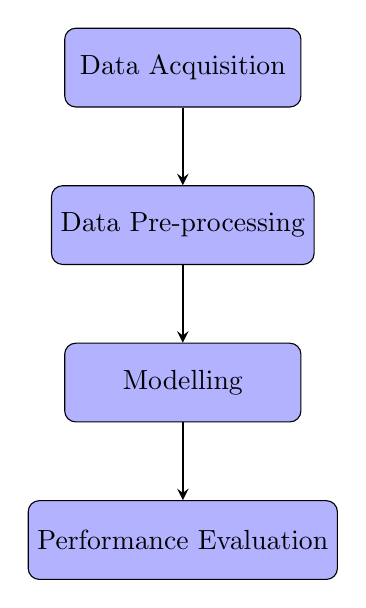
\begin{tikzpicture}[node distance=2cm]
        \node (start) [startstop] {Data Acquisition};
        \node (dc) [startstop, below of=start] {Data Pre-processing};
        \node (dpr) [startstop, below of=dc] {Modelling};
        \node (mtpe) [startstop, below of=dpr] {Performance Evaluation};
        \draw [arrow] (start) -- (dc);
        \draw [arrow] (dc) -- (dpr);
        \draw [arrow] (dpr) -- (mtpe);
    \end{tikzpicture}
    \caption{Traditional Machine Learning workflow}
\end{figure}

\newpage
\section{Bias}

Artificial Intelligence (AI) is undeniably a transformative force, poised to reshape multiple dimensions of the existence in profound ways. Its versatile applications extend far and wide, from refining and expediting decision-making processes to seamlessly automating mundane and repetitive tasks. In this ever-evolving landscape, AI systems are becoming increasingly integrated into daily experiences, orchestrating a paradigm shift in the way people interact with the world around them. 

However, amidst the excitement and optimism surrounding AI's potential, a growing concern resonates both within the AI community and society as a whole. This concern revolves around the pervasive issue of biases intricately woven into the very fabric of AI algorithms. 

These biases, often unintentional and subtle, can seep into AI systems through the data they are trained on and the methods employed to develop them. As AI systems learn from historical data, they may inadvertently inherit the prejudices and stereotypes present in those datasets. Consequently, these biases can manifest in various ways, perpetuating and amplifying societal inequalities. For example, in AI applications for hiring or lending, biases can result in unfair discrimination based on factors such as race or gender. In automated content recommendations, biases can reinforce echo chambers, limiting exposure to diverse perspectives and ideas. 

The consequences of these biases are far-reaching and profound. They not only undermine the ethical foundations of AI but can also erode trust in these technologies. As AI systems gain prominence in critical areas like healthcare, criminal justice, and education, the ramifications of bias become increasingly worrisome. 

Addressing bias in AI is a complex and ongoing challenge. It requires a multifaceted approach that encompasses not only improved data collection and curation but also transparency in AI decision-making processes. Researchers and engineers are working tirelessly to develop techniques for bias detection and mitigation. Additionally, there is a growing push for diverse representation in the AI development community to ensure that the creation of AI systems considers a wide array of perspectives. 

In conclusion, while the promise of AI is immense, the journey towards harnessing its potential responsibly and equitably is an imperative one. Moving forward in this AI-driven era, it is essential to remain vigilant in identifying and rectifying biases, ensuring that AI truly serves as a force for positive change in an always faster evolving world. \cite{10.1145/3308560.3317590}

\subsection{Understanding Bias in AI}

Bias in AI is a critical issue, signifying the presence of unjust and skewed representations or treatment of individuals or groups based on attributes such as race, gender, age, socioeconomic status, or other defining characteristics. These biases are deeply embedded in AI systems and can persist throughout their development and training processes. They arise from a variety of sources, including historical data imbalances, deeply ingrained societal prejudices, and imperfections in the algorithms themselves.

\subsection{Sources of Bias}

It's possible to establish 3 different sources of biases across several perspectives: historical, human and algorithmic perspective.

\begin{figure}[H]
    \centering
    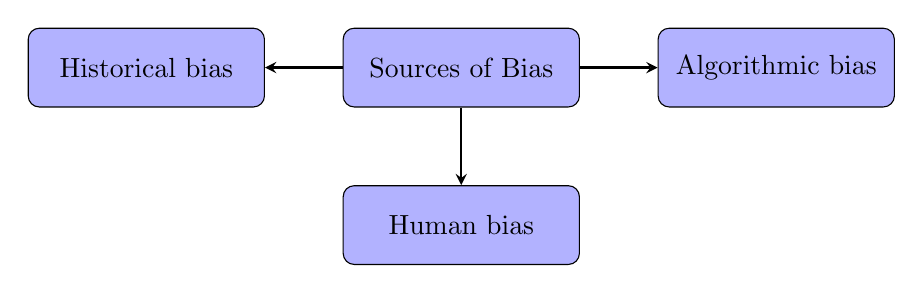
\begin{tikzpicture}[node distance=2cm]
        \node (start) [startstop] {Sources of Bias};
        \node (dc) [startstop, left of=start, xshift=-2cm] {Historical bias};
        \node (dpr) [startstop, below of=start] {Human bias};
        \node (mtpe) [startstop, right of=start, xshift=2cm] {Algorithmic bias};
        \draw [arrow] (start) -- (dc);
        \draw [arrow] (start) -- (dpr);
        \draw [arrow] (start) -- (mtpe);
    \end{tikzpicture}
    \caption{Sources of bias}
\end{figure}

\subsubsection{Historical bias} 

The issue of bias originating from historical data is a critical and intricate challenge that looms large in the landscape of machine learning. When machine learning models are trained on datasets culled from the annals of history, they inevitably inherit the biases and patterns encoded within that data. These historical biases, often a reflection of deeply ingrained societal prejudices and structural inequalities, can persist and intensify when the model is operationalized. \cite{10.1145/3308560.3317590}

Consider a scenario where historical data contains systemic biases against specific demographics, such as gender, race, or other socio-demographic attributes. The machine learning model, in its quest to optimize performance, dutifully replicates and perpetuates these biases in its predictions and decision-making processes. The consequence of this perpetuation is the perpetuation of historical injustices, potentially leading to the endorsement of discriminatory practices and the exacerbation of preexisting societal inequalities, significantly disadvantaging certain groups. 

Effectively addressing bias originating from historical data necessitates a multidimensional approach, coupled with proactive measures.

\begin{enumerate}

    \item The first step involves diligent data preprocessing techniques aimed at the identification and subsequent mitigation of bias-laden elements within the dataset. These techniques span a spectrum from data re-sampling to re-weighting and data augmentation, designed to restore balance and fairness.

    \item Simultaneously, interventions in algorithmic fairness are introduced to the machine learning process. These interventions encompass a range of techniques, including re-weighting of training instances, the introduction of fairness constraints, and adversarial debiasing methods, all aimed at guiding the model toward making fair and equitable predictions. 

    \item Moreover, the journey toward equitable AI is an ongoing one, requiring constant vigilance. Continuous monitoring and adjustment of models, often in real-time, become imperative to ensure that fairness is upheld and biased outcomes are identified and rectified. 

\end{enumerate}

Ultimately, the overarching goal is to foster a future where machine learning not only learns from historical data but actively works to transcend the bonds of bias. In this vision, AI systems operate as champions of fairness and social justice, contributing to the construction of a more equitable and just society where decisions and predictions are untainted by historical prejudices. This endeavor is not just a technical challenge but a moral imperative, driving the AI community to build a more equitable future for all.

\subsubsection{Human bias}

Bias introduced by human factors represents a pervasive and intricate challenge within the realm of machine learning. It is essential to understand that human bias, which can emanate from societal, cultural, or personal beliefs and attitudes, has the potential to inadvertently permeate the entire spectrum of the machine learning pipeline. This influence spans from the initial stages of data collection and annotation to the model training and decision-making processes. 

Human bias can manifest in multifarious ways, thereby complicating the quest for fair and unbiased machine learning models. These manifestations may include the biased selection of training data, subjectivity in annotations, or implicit prejudices that insidiously seep into the very fabric of algorithm design and evaluation. When humans are intricately involved in the decision-making processes or contribute to the development of algorithms, their biases, often unperceived, can become unintentionally embedded in the model. This results in a cascade of skewed predictions and the inadvertent reinforcement of preexisting societal inequalities. \cite{https://doi.org/10.1002/widm.1356} 

The recognition and mitigation of human bias represent an imperative for the development of equitable and just machine learning models. This mission encompasses several facets:

\begin{enumerate}

    \item First and foremost, it demands an elevated level of awareness within the machine learning community and society at large. Recognizing the potential pitfalls of human bias is a crucial step toward addressing them. 

    \item Promoting diversity and inclusion, both in the workforce and in the datasets used for model training, is instrumental in countering human bias. Diverse perspectives and a multiplicity of experiences contribute to a more comprehensive and unbiased understanding of the world. 

    \item Moreover, practical measures are implemented to detect and mitigate bias throughout the machine learning pipeline. This includes strategies ranging from fairness-aware machine learning algorithms to post-processing techniques that rectify biased predictions. 

    \item The journey toward mitigating human bias is continuous and iterative. Machine learning practitioners continually refine their algorithms to minimize the impact of human bias and ensure that their models contribute to a more equitable and unbiased society. 

\end{enumerate}

The ultimate goal is to harness the transformative potential of machine learning while eliminating the inadvertent perpetuation of human biases, thereby ushering in a more equitable and just era in technological advancement.

\subsubsection{Algorithmic bias}

Algorithmic bias, an intrinsic challenge in the domain of machine learning, underscores the presence of inherent biases that can manifest in the design, development, and deployment of machine learning algorithms. These biases, often unintended, can originate from a myriad of sources, encompassing factors such as biased training data, skewed feature selection, or implicit assumptions woven into the algorithm's development process. 

Algorithmic bias possesses the insidious potential to perpetuate and magnify preexisting societal prejudices and disparities, culminating in outcomes that are patently unfair and discriminatory. Consider the scenario in which a machine learning model is trained on historical data that inherently encapsulates societal biases. The model, in its endeavor to optimize predictive accuracy, inadvertently assimilates and reinforces these biases. The result is an algorithm that produces predictions and decisions that are tinged with bias, potentially aggravating societal inequalities and offering unequal treatment to specific groups. \cite{10.1145/2983270} 

The algorithmic bias mitigation requires several steps:

\begin{enumerate}

    \item Addressing algorithmic bias is a pivotal imperative when striving to construct equitable and just AI systems. This undertaking encompasses a comprehensive scrutiny of the entire machine learning pipeline, from data collection to model development and deployment. It commences with the meticulous assessment and rectification of bias within training data, aiming to restore balance and fairness. 

    \item The integration of fairness-aware algorithms within the machine learning process is crucial. These algorithms are deliberately designed to recognize and rectify biases, offering a safeguard against discriminatory predictions and decisions.

    \item Transparency and fairness represent integral aspects of the decision-making process. The incorporation of these elements ensures that algorithms operate equitably, are devoid of bias, and actively promote fairness and equal treatment for all individuals, irrespective of their backgrounds. 

\end{enumerate}

In essence, the mission of addressing algorithmic bias is pivotal for harnessing the true potential of AI systems. It involves forging a future where AI, far from perpetuating biases, serves as a champion of fairness and social justice, contributing to the construction of an equitable and just society in the digital age.

\subsection{Example of Bias in AI}

\subsubsection{Race and Gender Bias in Facial Recognition} 

Race and gender bias in facial recognition technology is a pressing and deeply concerning issue that underscores the ethical complexities tied to the development of AI. Facial recognition systems, often trained on large datasets, inadvertently perpetuate biases present in these datasets, particularly biases related to race and gender. The lack of diversity in training data, which is predominantly skewed towards certain demographics, results in algorithmic bias, where the system may struggle to accurately recognize individuals from underrepresented racial or gender groups. \cite{https://doi.org/10.5281/zenodo.4050457}

Studies have provided compelling evidence that these systems are often more accurate for individuals with lighter skin tones compared to those with darker skin tones, demonstrating a clear racial bias. Similarly, gender recognition algorithms may exhibit inaccuracies, especially for gender-nonconforming individuals, further exacerbating biases. 

The consequences of these biases are wide-ranging and profound. For instance, in law enforcement applications, the use of facial recognition may lead to the disproportionate targeting and misidentification of individuals from minority communities, potentially resulting in wrongful arrests and increased surveillance. In commercial contexts, biased facial recognition can significantly impact hiring processes, access to services, and overall societal fairness, with far-reaching implications for individuals and communities.


\subsubsection{Criminal Justice Bias}

Criminal justice bias is a deeply ingrained issue within the legal system that manifests through unequal treatment of individuals based on their race, socioeconomic status, gender, and other factors. The criminal justice system should ideally operate on principles of fairness, justice, and equality before the law. However, biases at various stages of the criminal justice process, from policing and arrest to trial and sentencing, often lead to discriminatory outcomes. \cite{doi:10.1080/10345329.2019.1658694} 

Racial bias is a significant concern, with people of color, especially Black individuals and communities, experiencing disproportionately higher rates of arrest, harsher sentencing, and a lack of trust in the system. Discriminatory practices such as racial profiling and racial disparities in sentencing contribute to this bias. Socioeconomic bias is another critical factor, where individuals from marginalized and low-income communities may face prejudice in the form of limited access to legal resources and unequal treatment within the legal process. \cite{9660177}  

Gender bias is prevalent, particularly against women and gender-diverse individuals. Women can face stereotypes and discriminatory attitudes that affect their treatment by law enforcement, the courts, and correctional facilities. Additionally, biases against LGBTQ+ individuals can result in unfair treatment and disparities in the criminal justice system. \cite{gebru2020race} 

Addressing criminal justice bias necessitates comprehensive reform. This includes implementing policies to combat racial and socioeconomic disparities, providing anti-bias training to law enforcement, encouraging diversity within the legal profession, and promoting transparency and accountability in the criminal justice process. Legislation, sentencing reform, community engagement, and the support of marginalized communities are also vital steps toward achieving a fair and impartial criminal justice system that upholds the principles of equity and justice for all.


\subsubsection{Recruitment Bias}

Recruitment bias is a critical issue within the hiring process, where unconscious or conscious prejudices and preconceived notions influence decision-making during candidate selection. It manifests in various forms, such as racial, gender, age, socio-economic, educational, or even appearance-based biases, and can significantly impact the composition of the workforce. \cite{mujtaba2019ethical} 

One of the most prevalent forms of recruitment bias is racial or ethnic bias. Hiring decisions can be influenced by stereotypes, leading to the underrepresentation of certain racial or ethnic groups in the workplace. Similarly, gender bias can result in disparities in hiring and promotion opportunities, favoring one gender over another. Age bias often affects older candidates who may be overlooked in favor of younger, perceived to be more 'tech-savvy' individuals. 

Educational and socio-economic biases can also seep into the hiring process, where candidates from prestigious institutions or privileged backgrounds may be given preferential treatment. Appearance-based biases, although highly unfortunate, can influence decisions, impacting individuals based on their physical attributes, such as weight, height, or even hairstyle. 

Addressing recruitment bias requires a multipronged approach. Firstly, raising awareness and providing training on unconscious bias is essential for hiring teams. Implementing structured and standardized interview processes, blind recruitment techniques (removing personally identifiable information), and diverse interview panels can help mitigate biases. Moreover, organizations should focus on promoting diversity and inclusion, fostering a culture that values different perspectives and backgrounds, and monitoring and analyzing recruitment data to identify patterns of bias. Striving for fairness and inclusivity in the hiring process not only leads to a more diverse workforce but also improves organizational innovation, creativity, and overall success.

\section{Fairness} 

The pursuit of fairness within AI systems represents a dynamic and indispensable area of focus within the ever-expanding realm of artificial intelligence. At its core, fairness underscores an ethical and moral imperative to ensure that AI technologies and algorithms treat all individuals with equitable respect, devoid of bias or discrimination. As AI increasingly penetrates diverse facets of society, from decision-making processes to job recruitment, lending, and law enforcement, the salience of fairness is unequivocal. 

The pursuit of fairness in AI is an all-encompassing endeavor, entailing an array of considerations that orbit around the ambition to eliminate bias predicated on attributes such as race, gender, age, ethnicity, and socio-economic status. Bias in AI manifests in multifarious ways, originating from the training data's inherent biases or the algorithms themselves. Fair AI systems, therefore, endeavor to minimize these biases, upholding the principles of impartiality and justice in the outcomes they produce. 

In the quest for fairness, various fairness metrics and criteria have emerged, serving as quantifiable benchmarks for assessing the equity of AI systems. These include disparate impact, equal opportunity, and demographic parity. 

\begin{itemize}

    \item Disparate impact assesses the differential impact an AI system has on distinct demographic groups

    \item Equal opportunity guarantees that the probability of a positive outcome remains consistent across all demographic segments

    \item Demographic parity, on the other hand, centers on the proportional representation of various groups within AI-generated outcomes

\end{itemize}

Addressing fairness within AI systems necessitates the employment of an assortment of techniques. This involves pre-processing data to ameliorate biases, the modification of algorithms to instill them with fairness-awareness, and post-processing methods to ensure that outcomes are equitable. Furthermore, transparency and explainability are pivotal features of AI models, facilitating a deeper understanding of potential biases and nurturing trust in the technology. 

Emphasizing the ethical dimension, the pursuit of fairness in AI systems transcends the confines of technical solutions. It necessitates the active involvement of stakeholders, the incorporation of diverse perspectives, and a steadfast commitment to adhering to guidelines and regulations that prioritize fairness and impartiality. 

In essence, the journey to achieve fairness in AI systems is an ongoing and multifaceted odyssey, demanding relentless research, interdisciplinary collaboration, and unwavering ethical vigilance. The ultimate objective is the creation of AI technologies that steadfastly uphold the principles of fairness, contributing to a more inclusive, just, and equitable society. The continued pursuit of fairness in AI is not just a technical endeavor but a moral imperative, shaping the future of technology and its impact on society.

\subsection{Fairness Techniques in AI}

\subsubsection{Pre-processing}

Pre-processing focuses on the pre-processing phase, an integral component of AI system development, is dedicated to the meticulous handling of data before it is utilized in the training of an AI model. This stage assumes paramount importance as it lays the foundation for equitable and unbiased AI systems, ensuring that the data used is both balanced and representative of the rich diversity inherent in the population. 

The objective of pre-processing is to rectify any imbalances, biases, or irregularities in the data, aiming to foster an environment where the AI model can operate without predisposition. The use of common pre-processing techniques is pivotal to this endeavor. These techniques encompass oversampling and undersampling, which seek to redress the imbalance in the distribution of data across various classes or groups. 

Additionally, pre-processing includes the meticulous removal of noise from the data. Noise, in this context, refers to extraneous or irrelevant information that could distort the model's learning process. The elimination of such noise serves to enhance the data's signal-to-noise ratio, improving the model's ability to discern meaningful patterns. 

Furthermore, the creation of balanced synthetic datasets is a valuable technique within the pre-processing repertoire. This involves the generation of new data points, often through the extrapolation of existing data, with the goal of augmenting the representation of underrepresented classes or groups. 

In summation, pre-processing is the cornerstone of equitable and unbiased AI system development. It encompasses a suite of techniques designed to foster balanced and representative data, enabling AI models to operate with impartiality and fairness, contributing to more equitable and unbiased outcomes. handling the initial data before it is used to train the AI model. This stage is crucial to ensure that the data is balanced and representative of the diversity in the population. Common pre-processing techniques include oversampling, undersampling, noise removal from the data, and creating balanced synthetic datasets.

\subsubsection{In-processing}

In-processing techniques represent a focused and interventionist approach that takes place directly during the model training phase. This method aims to instill fairness into the AI model at its core, ensuring equitable and unbiased outcomes. It is a precise and intricate strategy designed to mitigate bias and discrimination within the model's decision-making processes. 

One prominent in-processing technique involves the application of regularization methods. Regularization techniques are instrumental in penalizing the model when it demonstrates a discriminatory inclination, particularly with regard to certain sensitive features, such as gender or ethnic origin. By imposing penalties, the model is encouraged to refrain from exhibiting bias and to generate fair and impartial predictions. 

Another facet of in-processing techniques involves the alteration of cost functions. By modifying the cost functions, the model's training process is steered toward fairness. This modification ensures that the model pays a cost for making biased predictions, thereby incentivizing it to provide equitable treatment across different categories. 

In addition to regularization and cost function adjustments, in-processing techniques may encompass the manipulation of the model's predictions themselves. This manipulation can be guided by fairness constraints, ensuring that the model's outputs adhere to the principles of fairness and impartiality, especially concerning sensitive attributes. 

In summary, in-processing techniques serve as a focused and critical juncture in the quest for fairness within AI models. By intervening directly during the model training phase, these techniques work toward equitable and unbiased outcomes, promoting the development of AI technologies that contribute to a more fair and inclusive society.

\subsubsection{Post-processing}

Post-processing unfolds after the model has been meticulously trained and has generated predictions. This phase assumes the role of a corrective and fine-tuning mechanism, primarily focusing on adjustments and modifications to the model's predictions with the overarching objective of ensuring fairness and equity. 

One key facet of post-processing involves the application of realignments or adjustments to the model's predictions. These realignments are designed to rectify any unjustified disparities among demographic groups, ensuring that the model's outcomes are equitable and devoid of bias. This process may entail recalibrations or other transformative actions applied to the model's results to mitigate any latent biases that may have emerged during the training process. 

The successful implementation of post-processing techniques hinges on a profound understanding of the specific fairness challenges inherent in both the data and the models. This demands a nuanced comprehension of the intricacies of the data, including potential sources of bias and discrimination. Furthermore, it requires a comprehensive grasp of the model's inner workings, discerning where and why biases may have arisen. 

Ongoing evaluation represents an indispensable element of the post-processing phase. Continual assessments and audits are essential to ensure that AI models adhere to ethical standards and actively promote fairness. This continuous vigilance and adjustment are pivotal in fostering AI technologies that contribute to the construction of a more equitable and just society. 

In essence, post-processing represents the culmination of efforts to instill fairness within AI models, serving as the final safeguard against bias and discrimination in the model's predictions.

\subsection{Pre-processing Techniques for Addressing Fairness in AI}

Pre-processing techniques are applied before the training step, in orer to try to avoid bias and guarantee fairness to the data on which the ML models are trained. Several techniques can be emplyed in the pre-processing step:

\subsubsection{Oversampling and Undersampling}

Oversampling and undersampling are techniques used to address class imbalance, where one class significantly outnumbers the others in a dataset. In the context of fairness, these techniques are employed to ensure that the AI model is not biased towards the majority class and that the predictions are fair and equitable for all classes, particularly when sensitive attributes like race, gender, or ethnicity are involved. \cite{9442706}

\begin{enumerate}

    \item \emph{Oversampling}

    \begin{itemize}

        \item \emph{Definition:} Oversampling involves increasing the number of instances in the minority class by generating synthetic samples or replicating existing ones.
        
        \item \emph{Fairness Context:} Oversampling aims to boost the representation of underrepresented groups, promoting fairness and equal consideration of all groups. It prevents the model from exhibiting bias towards the majority group.
    
    \end{itemize}

    \item \emph{Undersampling}

    \begin{itemize}

        \item \emph{Definition:} Undersampling involves reducing the number of instances in the majority class by removing samples, ideally in a strategic and unbiased manner.
        
        \item \emph{Fairness Context:} Undersampling can be employed to level the playing field by reducing the dominance of the majority group. This ensures that the model's predictions are not disproportionately influenced by the majority group, promoting fairness in the model's outcomes.
    
    \end{itemize}

\end{enumerate}

\subsubsection{Noise Removal}

Noise removal in the context of fairness typically refers to the process of identifying and mitigating the effects of noisy or incorrect data points that may introduce biases or distortions in the data used to train or evaluate machine learning models. In fairness considerations, noise removal plays a crucial role in ensuring that the AI system's predictions and decisions are as accurate and unbiased as possible, particularly when sensitive attributes like race, gender, or ethnicity are involved. \cite{NEURIPS2019_8d5e957f}

\subsubsection{Data Augmentation}

Data augmentation is a technique often used in machine learning and data preprocessing to artificially increase the size and diversity of a training dataset by generating new data points based on the existing ones. In the context of fairness, data augmentation can play a crucial role in addressing imbalances and biases in the data, particularly when sensitive attributes are involved. Here's how data augmentation can be applied in the context of fairness:

\begin{enumerate}

    \item \emph{Generating Additional Data for Underrepresented Groups}
    
    \begin{itemize}

        \item In scenarios where certain groups or classes are underrepresented in the training data, data augmentation techniques can be used to create additional examples for those groups. \cite{sharma2020data}
    
    \end{itemize}
    
    \item \emph{Balancing Class or Group Representation}
    
    \begin{itemize}
        
        \item Data augmentation can be employed to balance class or group representation in the training data. By creating synthetic data points for underrepresented groups, it helps ensure that the model is not biased towards majority groups.
    
    \end{itemize}
    
    \item \emph{Feature Engineering for Fairness}
    
    \begin{itemize}
        
        \item Data augmentation can also involve feature engineering that considers sensitive attributes. For example, it can create new features that better capture the nuances and characteristics of underrepresented groups. \cite{10.14778/3461535.3463474}
    
    \end{itemize}
    
    \item \emph{Fair Data Augmentation}
    
    \begin{itemize}
    
        \item In the fairness context, it's important to ensure that data augmentation techniques do not introduce additional biases. Care should be taken to create synthetic data that aligns with the fairness and equity goals of the AI system. \cite{10.1145/3531146.3534644}
    
    \end{itemize}

\end{enumerate}

\subsubsection{Bias Mitigation Algorithms}

Bias mitigation in the context of fairness refers to the process of identifying, reducing, or eliminating biases within machine learning models and algorithms, particularly those that could lead to unfair or discriminatory outcomes, often associated with sensitive attributes like race, gender, age, or ethnicity. The goal of bias mitigation is to ensure that AI systems provide equitable and unbiased predictions and decisions for all individuals or groups.

\subsubsection{Sensitive Attribute Removal or Neutralization}

In some cases, sensitive attributes (e.g., race, gender) can be removed from the dataset or transformed into more neutral representations. This prevents the model from relying on these attributes to make predictions, promoting fairness. \cite{NEURIPS2021_64ff7983}

These pre-processing techniques are essential steps in the AI development pipeline to ensure that the subsequent models are fair, unbiased, and capable of providing equitable outcomes across various demographic categories.

\subsection{In-processing Techniques for Addressing Fairness in AI}

In-processing techniques aim to mitigate fairness issues directly during the model training phase, influencing the learning process to ensure fairness in model predictions. These approaches target bias reduction and fairness promotion within the model's decision-making process. Several techniques can be employed during model training to achieve fairness:

\subsubsection{Regularization}

Regularization  aims to address and mitigate potential biases within models, particularly when sensitive attributes like race, gender, or ethnicity are involved. Regularization techniques work by adding constraints or penalties to the model's training process to reduce the impact of sensitive attributes on predictions and ensure that fairness is maintained. \cite{6137441}

\subsubsection{Reweighting Training Samples}

Reweighting training samples is a technique used to address bias and promote fairness in machine learning models, particularly when sensitive attributes are involved. This approach involves assigning different weights to training samples to influence the learning process of the model in a way that mitigates bias and ensures that predictions are more equitable. \cite{10.1145/3178876.3186133}

\subsubsection{Prejudice Remover Regularizer}

The Prejudice Remover Regularizer is a technique used to mitigate bias and promote equitable outcomes in machine learning models. It's a form of regularization that aims to reduce discrimination by encouraging the model to make predictions that are less influenced by sensitive attributes such as race, gender, or ethnicity. \cite{10.1007/978-3-642-33486-3_3}

\subsubsection{Demographic Parity Loss}

The Demographic Parity Loss is a fairness metric and regularization technique used to promote fairness and reduce bias, particularly with regard to sensitive attributes like race, gender, or ethnicity. It is designed to ensure that the predictions made by a model are distributed equally or fairly across different demographic groups. \cite{jiang2022generalized}

\subsubsection{Fair Adversarial Training}

Fair adversarial training is a technique used in the context of fairness to reduce bias and discrimination in machine learning models, particularly when sensitive attributes like race, gender, or ethnicity are involved. This approach incorporates adversarial networks into the training process to promote fairness and equitable outcomes. \cite{pmlr-v139-xu21b}

These in-processing techniques are vital tools in promoting fairness within AI models. Integrating them appropriately during model training can significantly contribute to reducing biases and achieving equitable outcomes across various demographic categories.

\subsection{Post-processing Techniques for Addressing Fairness in AI}

Post-processing techniques are applied after the model has been trained and predictions have been generated. Their purpose is to rectify any biases or disparities in the model's outputs and ensure fairness in the final outcomes. Several techniques can be employed during post-processing to promote fairness:

\subsubsection{Threshold Adjustments}

Threshold adjustment is a technique used to promote equity and reduce bias in machine learning models, especially in scenarios where sensitive attributes like race, gender, or age play a significant role. It involves modifying the decision threshold that determines whether a model's output is classified as a positive or negative prediction. This adjustment aims to balance the rates of false positives and false negatives across different demographic or group categories, ensuring that all groups are treated more fairly. \cite{10.1145/3447548.3467251}

\subsubsection{Additive Counterfactuals}

Additive counterfactual explanations in the context of fairness refer to a method used to assess and promote fairness in machine learning models. Counterfactual explanations are designed to provide insights into the impact of sensitive attributes on model predictions and help identify potential bias or discrimination. The additive aspect suggests that changes are made to the original input to create counterfactual scenarios, allowing for a better understanding of the fairness implications. \cite{NIPS2017_a486cd07}

\subsubsection{Equalized Odds Post-processing}

Equalized Odds Post-processing is a technique used to mitigate bias and promote equal treatment in machine learning models, particularly in scenarios involving binary classification tasks. This technique is applied after a model has made predictions and aims to adjust those predictions to ensure that equal error rates are achieved across different demographic or group categories. \cite{10.1145/3442188.3445902}

These post-processing techniques are crucial in rectifying biases and promoting fairness in AI models. Utilizing them effectively can lead to more equitable outcomes and decisions across various demographic categories.

\section{Fair-by-Design}

Fair-by-design methods represent a proactive approach to addressing bias and promoting fairness in machine learning and artificial intelligence systems from their inception. These methods aim to embed fairness considerations into the design and development of algorithms and models to prevent bias from emerging in the first place. 

There are several key aspect to consider during the development of a Fair-by-Design method:

\begin{itemize}

    \item A careful curation and preprocessing of training data to mitigate biases that might be present. For instance, techniques for re-sampling, re-weighting, and data augmentation can be employed to balance underrepresented groups in the data.

    \item It's required the modification of algorithms to incorporate fairness-awareness. This can be achieved through the introduction of fairness constraints during the training process or through adversarial debiasing techniques.

    \item Post-processing methods are often utilized to ensure that the outcomes of machine learning models are equitable. These methods can include adjusting the model's predictions to reduce disparities between different groups.

\end{itemize}

The ultimate goal of fair-by-design methods is to create AI systems that, from their very conception, are inherently fair and unbiased. By considering fairness as a fundamental design principle, it's possible to work towards eliminating discriminatory effects in AI systems, contributing to a more equitable and just technological landscape. 

\section{Fairness notions}
\label{section:fairness_notions}

Fairness notions serve as the foundational pillars that define the ethical considerations and objectives guiding the development of AI systems within the Fair-by-Design workflow. These notions articulate specific principles for mitigating bias and promoting fairness, each with its unique characteristics and mathematical underpinnings.

\subsection{Demographic Parity}

Demographic Parity represents a fundamental fairness notion that addresses the equal representation of protected groups across different outcomes. In a binary classification context, it can be expressed as:

\[ P(\hat{Y} = 1 | A = a) = P(\hat{Y} = 1), \]

where \( \hat{Y} \) denotes the predicted outcome, \( A \) is the protected attribute, and \( a \) signifies a specific value of the protected attribute. The goal of Demographic Parity is to ensure that the distribution of positive outcomes is consistent across various demographic groups. While conceptually straightforward, Demographic Parity may overlook nuances in individual experiences and predictive accuracy.

\subsection{Equalized Odds}

Equalized Odds is a fairness notion that focuses on balancing the true positive and false positive rates across protected groups. Mathematically, it can be formalized as:

\[ P(\hat{Y} = 1 | A = a, Y = y) = P(\hat{Y} = 1 | Y = y), \]

where \( Y \) represents the true outcome. Equalized Odds strives to rectify disparities in prediction accuracy between protected groups, ensuring that both favorable and unfavorable outcomes are predicted with similar precision. This notion addresses concerns related to disparate error rates and aims to provide equal predictive performance for different demographic groups.

\subsection{Individual Fairness}

Individual Fairness introduces a nuanced dimension by emphasizing the fair treatment of similar individuals, irrespective of their protected attributes. While challenging to formalize precisely, it can be understood as:

\[ d(x, x') \leq \epsilon \Rightarrow |P(\hat{Y} = 1 | X = x, A = a) - P(\hat{Y} = 1 | X = x', A = a)| \leq \delta, \]

where \( d(x, x') \) measures the similarity between instances \( x \) and \( x' \), and \( \epsilon \) and \( \delta \) are predefined thresholds. Individual Fairness recognizes the unique characteristics of each instance and aims to ensure comparable treatment for similar individuals.

\subsection{Group Fairness}

Group Fairness extends fairness considerations to demographic groups, focusing on statistical parity in predicted outcomes. Formally, it can be expressed as:

\[ P(\hat{Y} = 1 | A = a) = P(\hat{Y} = 1 | A = a'), \]

where \( a \) and \( a' \) denote different values of the protected attribute. Group Fairness advocates for equitable treatment at the collective level, ensuring parity in the overall distribution of predicted outcomes among various demographic groups.

\section{Fairness metrics}
\label{section:metrics}

Fairness metrics play a crucial role in evaluating the performance of AI systems and ensuring equitable outcomes for diverse groups. These metrics provide quantitative measures to assess and mitigate bias within machine learning models. In this section, it will explored the general concept of fairness metrics and delve into three specific metrics: disparate impact, equalized odds, and demographic parity.

\subsection{General Overview}

Fairness metrics are quantitative tools designed to assess the impact of AI systems on different demographic groups. They help identify and address biases in model predictions, ensuring that the system does not disproportionately favor or disadvantage specific groups based on protected attributes such as race, gender, or age.

Common fairness metrics include disparate impact, equalized odds, demographic parity, and many others. These metrics are instrumental in evaluating the fairness and ethical implications of AI models, particularly in applications like hiring, lending, and education.

\subsection{Disparate Impact}

\emph{Definition:}

Disparate impact measures the ratio of favorable outcomes for different demographic groups. It highlights situations where a particular group experiences a disproportionately adverse impact compared to others.

\emph{Calculation:}
\[ DI = \frac{Pr(Y = 1|A=a)}{Pr(Y = 1|A=b)} \]

Where:
\begin{itemize}
    \item \( Y \) is the predicted outcome,
    \item \( A \) is the sensitive attribute (e.g., gender, race),
    \item \( a \) and \( b \) represent different values of the sensitive attribute.
\end{itemize}

\emph{Interpretation:}

A disparate impact value close to 1 indicates fairness, while values significantly deviating from 1 suggest potential bias.

\subsection{Equalized Odds}

\emph{Definition:}

Equalized odds ensures that the true positive rate and false positive rate are similar across different demographic groups. This metric focuses on achieving parity in both the benefits and errors of the model for different groups.

\emph{Calculation:}

\[ \text{True Positive Rate (TPR)} = \frac{Pr(\hat{Y} = 1|Y = 1, A = a)}{Pr(Y = 1|A = a)} \]
\[ \text{False Positive Rate (FPR)} = \frac{Pr(\hat{Y} = 1|Y = 0, A = a)}{Pr(Y = 0|A = a)} \]

\emph{Interpretation:}

Equalized odds is achieved when the TPR and FPR are approximately equal across all demographic groups.

\subsection{Demographic Parity}

\emph{Definition:}

Demographic parity requires that the proportion of positive outcomes is the same for all demographic groups, regardless of the sensitive attribute.

\emph{Calculation:}

\[ DP = Pr(\hat{Y} = 1|A = a) - Pr(\hat{Y} = 1|A = b) \]

\emph{Interpretation:}

A value close to 0 indicates fairness, suggesting that the model's predictions are not influenced by the sensitive attribute.

\section{Fairlearn Library}
\label{section:fairlearn}

Fairlearn is a powerful and versatile open-source Python library developed to address fairness concerns in machine learning models. Recognizing the importance of mitigating biases and ensuring equitable outcomes, Fairlearn provides a comprehensive set of tools, algorithms, and metrics designed to facilitate fairness-aware model development and evaluation.

\subsection{Key Features of Fairlearn}

Fairlearn offers a range of key features that empower researchers and practitioners to assess and enhance the fairness of their machine learning models:

\subsubsection{Fairness Metrics}

The library includes a diverse set of fairness metrics that enable quantitative assessment of bias and disparity in model predictions. Metrics such as disparate impact, equalized odds, and demographic parity provide insights into the impact of model decisions on different demographic groups.

\subsubsection{Algorithms}

Fairlearn incorporates fairness algorithms tailored for pre-processing, in-processing, and post-processing stages of the machine learning pipeline. These algorithms aim to mitigate biases and promote fairness in model predictions, offering flexibility for users to choose and integrate the most suitable techniques for their specific applications.

In conclusion, fairness in AI is not just an ethical necessity but a fundamental requirement for fostering trust and ensuring the responsible and equitable deployment of AI systems. Moving into the evolving landscape of AI, the collective efforts must prioritize fairness to harness the true potential of AI for the greater good.
%Write background here.

%This section is likely to contain a lot of citations.
%
%For instance in \cite{AnzengruberSocInfo2013} the authors propose a novel means for tackling with the problem of preventing bad things from happening.


%----------------------------------------------------------------------------------------
\chapter{Contribution} % possible chapter for Projects
\label{chap:contribution}

\section{Introduction to the Fair-by-Design Workflow}
\label{section:workflow-introduction}

In recent years, heightened scrutiny of the ethical implications associated with artificial intelligence (AI) and machine learning (ML) systems has arisen in response to the escalating influence of these technologies, particularly in domains where consequential decisions profoundly impact individuals' lives. The evolving landscape of AI ethics necessitates a conscientious examination of the ethical dimensions embedded in the development and deployment of these systems.

Amid this multifaceted ethical discourse, the imperative of integrating fairness into the fabric of AI design has emerged as a paramount consideration. The principle of fairness, when applied as a foundational element in the design process, underscores the need for AI systems to produce outcomes that are not only accurate and efficient but also just and equitable. Achieving fairness in AI development demands a comprehensive and deliberate approach, one that transcends mere post hoc considerations by embedding fairness principles from the very inception of the design process.

The conceptual framework of a Fair-by-Design (FBD) workflow encapsulates a meticulous set of principles and procedural steps, each strategically devised to ensure the attainment of equitable and unbiased outcomes throughout the entire lifecycle of an AI system. This includes not only the initial design and development phases but also extends to the implementation, deployment, and ongoing monitoring stages. The iterative nature of this workflow acknowledges the dynamic interplay between ethical considerations and technological advancements, emphasizing the continuous reassessment and refinement of fairness strategies.

By adopting a Fair-by-Design approach, stakeholders in AI development, ranging from researchers and engineers to policymakers and end-users, commit to a shared responsibility for cultivating a technological landscape where the ethical imperatives of fairness and equity are not afterthoughts but integral components steering the trajectory of AI systems towards societal benefit and justice. In essence, the pursuit of ethical AI underscores not only the advancement of technological capabilities but also the conscientious stewardship of these capabilities to ensure they align with ethical norms and societal values.


\subsection{Principles of Fair-by-Design Workflow}
\label{subsection:workflow-principles}

\begin{enumerate}[label=\arabic*.]
    \item \emph{Proactive Fairness Integration:}
    
    \begin{itemize}
       
        \item The cornerstone of the Fair-by-Design workflow lies in the proactive embedding of fairness considerations at the genesis of the design process, diverging from conventional practices where fairness is often retroactively addressed after system implementation.
        
        \item This proactive approach marks a transformative shift in the landscape of algorithmic development, underscoring the ethical imperative of forethought in anticipating and mitigating biases.
        
        \item Seamless integration of fairness into the initial design stages aims to forestall the emergence of discriminatory outcomes, establishing a bedrock rooted in equitable principles.
        
        \item Beyond its alignment with ethical standards, this proactive integration streamlines the developmental trajectory, fostering a more responsible and inclusive machine learning environment.
       
        \item This meticulous attention to fairness from the inception reflects a commitment to ethical AI practices that transcend mere compliance, embodying a conscientious endeavor to uphold societal values and ensure the equitable treatment of diverse individuals impacted by AI systems.
   
    \end{itemize}

    \item \emph{Transparency and Explainability:}
    
    \begin{itemize}
        
        \item The Fair-by-Design workflow places a premium on transparent documentation of design decisions and algorithmic choices, considering it a fundamental pillar of its ethical framework.
       
        \item Meticulous documentation serves as a deliberate and strategic endeavor to enhance accountability and foster trust among stakeholders.
       
        \item Each decision, ranging from the selection of specific algorithms to the fine-tuning of parameters, is comprehensively recorded, creating a clear and accessible trail of the workflow's development trajectory.
       
        \item This commitment to transparency is deeply rooted in the conviction that open communication of design rationales and choices cultivates a sense of reliability and confidence among stakeholders.
       
        \item By actively promoting transparency, the Fair-by-Design workflow contributes to the creation of a trustworthy and ethically grounded landscape for the deployment of machine learning systems.
       
        \item The deliberate and open documentation not only satisfies ethical considerations but also facilitates a more robust understanding of the system's inner workings, empowering stakeholders to engage meaningfully in the ongoing dialogue surrounding the ethical dimensions of AI technologies.
    
    \end{itemize}

    \item \emph{User-Centered Approach:}
   
    \begin{itemize}
      
        \item Within the Fair-by-Design workflow, the integration of diverse perspectives transcends a passive consideration; it stands as a proactive and integral aspect of the design process.
      
        \item The voices and perspectives of end-users and relevant stakeholders are not only actively sought but thoughtfully incorporated from the early stages of system design.
      
        \item This inclusive approach is designed to ensure that the developed system is finely tuned to the diverse needs, expectations, and concerns of its user base.
     
        \item Stakeholder engagement takes on various forms, ranging from surveys and interviews to collaborative workshops.
      
        \item These mechanisms allow for a comprehensive understanding of the social, cultural, and ethical dimensions that may influence system usage.
       
        \item Actively involving end-users and stakeholders in the design process serves a dual purpose: promoting inclusivity and enhancing the likelihood of developing a system that genuinely serves and respects the interests of its users.
       
        \item This user-centered approach is not merely a procedural step but a foundational commitment to creating AI systems that align with the values and requirements of the communities they impact.
    
    \end{itemize}

    \item \emph{Continuous Monitoring and Iterative Development:}
    
    \begin{itemize}
     
        \item Beyond the initial implementation, the Fair-by-Design system adopts a vigilant and continuous monitoring regimen, constituting a pivotal component of its iterative workflow.
     
        \item This meticulous monitoring process is crafted to detect and address emerging fairness issues that may manifest during system operation.
     
        \item Leveraging advanced monitoring tools and techniques, the workflow ensures that the system's performance is regularly assessed in real-world scenarios.
      
        \item This proactive approach enables the timely identification of potential biases or disparities, allowing for the swift implementation of corrective measures.
     
        \item The iterative nature of the workflow is a testament to its adaptability, facilitating ongoing refinements to ensure that the system evolves in response to changing dynamics and user experiences.
     
        \item This commitment to continuous monitoring and improvement underscores the Fair-by-Design philosophy: an emphasis not only on achieving fairness at a single point in time but on actively maintaining and enhancing fairness throughout the system's entire lifecycle.
      
        \item By embracing a dynamic and iterative model, the Fair-by-Design workflow remains resilient, ensuring that it remains responsive to the evolving landscape of ethical considerations and technological advancements in artificial intelligence.
   
    \end{itemize}

\end{enumerate}

\section{Steps to Implement a Fair-by-Design Workflow}
\label{section:steps}

\begin{enumerate}

    \item \emph{Objective Definition:} Clearly articulate the objectives of the system or process being designed, emphasizing the importance of fairness.

    \item \emph{Data Collection:} Determine the types of data needed for the application, establish ethical data collection protocols.

    \item \emph{Data pre-processing:} Prepare the data for the fairness algorithm, through data cleaning and featyre engineering
    
    \item \emph{Algorithmic Design and Definitions:} Define and implement fairness-enhancing algorithms across pre-processing, in-processing, and post-processing stages. Provide detailed definitions and explanations for each algorithm.

    \item \emph{Model training and evaluation:} Define the training step, performs the training tuning certain parameters and provides an evaluation of the performances of the models based on accuracy and fairness metrics.

    \item \emph{Model deployment:} Define the change of the environment of the model from a development environment to real world application environment.

\end{enumerate}

\textbf{********************ADD FIGURE HERE***************************+}





\chapter{Validation}
\label{chap:validation}

\section{Introduction}
This chapter unfolds as a meticulous exploration into the performance and reliability of the Fair-by-Design workflow. To conduct a thorough assessment, the Educational Dataset obtained by ULL has been strategically chosen as the testing ground. This dataset, rich in attributes that can be both protected and impactful on students' performance in a specific subject, provides a nuanced platform for evaluating the workflow's effectiveness across various machine learning algorithms.

The central emphasis of this validation endeavor is to ascertain not only the accuracy and predictive capabilities of the implemented models but also the extent to which the Fair-by-Design workflow succeeds in fostering fairness. The Educational Dataset allows for a detailed examination of how different algorithms respond to the intricacies of real-world educational data, shedding light on the interplay between accuracy and fairness.

Throughout this chapter, the validation process unfolds systematically, encompassing diverse algorithms applied to the Educational Dataset. The goal is to detect both the strengths and potential limitations of the Fair-by-Design approach, providing valuable insights for its application in educational scenarios where the equitable treatment of students and the accuracy of predictions are of paramount importance. The subsequent sections detail the experimental setup, algorithmic choices, and the rigorous evaluation metrics employed to ensure a comprehensive understanding of the Fair-by-Design workflow's performance on the chosen educational dataset.

\section{Dataset description}

Before delving into the intricate details of the algorithm implementations presented earlier, it is imperative to provide a comprehensive overview of the dataset on which these algorithms have been applied. The chosen dataset for this work is the \emph{Canary Island Educational dataset}, an invaluable resource that underpins the empirical exploration of bias mitigation strategies in the context of the educational system in the Canary Islands. 

The Canary Island Educational dataset is a rich and expansive repository of information, meticulously compiled to capture various facets of the educational landscape within the Canary Islands. This dataset comprises the comprehensive census of students enrolled over four distinct academic years, offering a multifaceted glimpse into the educational ecosystem. 

The dataset encompasses a diverse array of attributes and data points, encapsulating critical information such as student demographics, academic performance, socioeconomic factors, and other pertinent variables. These attributes collectively provide a holistic perspective on the educational landscape, enabling a nuanced analysis of the factors that influence student outcomes and experiences. 

The temporal dimension of the dataset, spanning four academic years, further enriches the analytical potential. It allows for the investigation of temporal trends, shifts in educational policies, and the evolution of student characteristics over time. This temporal depth is particularly valuable when examining the efficacy of bias mitigation strategies, as it facilitates the assessment of their impact across different academic years. 

The Canary Island Educational dataset is not merely a repository of numbers and statistics; it is a window into the educational opportunities and challenges faced by students in the Canary Islands. By harnessing the insights gleaned from this dataset, it becomes possible to proactively address biases and promote equity within the educational system, ultimately striving for a more inclusive and just educational landscape.

\section{Precise Definition of Objectives}
\label{section:val_obj}

In this section, are meticulously outlined the objectives that intricately guide the Fair-by-Design workflow, with a primary focus on achieving effective prediction about the english level of each student while concurrently addressing fairness considerations and mitigating biases. The critical components encompass the meticulous identification of protected attributes, the strategic selection of fairness notions, and the corresponding choice of fairness metrics.

\subsection{Prediction Objective}

The overarching objective is to execute a fairness-driven classification task, discerning whether a student's english level is either above or under a certain threshold for each student enrolled in the 4 grade.

\subsection{Protected Attributes}

The identified protected attributes for scrutiny within the Fair-by-Design framework are the following:

\begin{itemize}

    \item sex

    \item capital island: if the student comes from the capital of the city

    \item public\textunderscore private: if the school is public or private
    
    \item mothly houseold income

    \item economic, social and cultural satus index

\end{itemize}

These attributes hold particular significance in the context of potential biases and fairness considerations.

\subsection{Fairness Notions}

To operationalize fairness, two distinct notions are employed, each serving specific objectives:

\begin{itemize}
    \item \emph{Demographic Parity:} The objective is to ensure a consistent distribution of predicted outcomes across different subgroups delineated by the protected attributes. This aligns with the broader goal of fostering equity in predictions.

    \item \emph{Group Fairness:} The goal is to guarantee equitable predictions within specific subgroups defined by protected attributes. This notion emphasizes the need for fairness at a more granular level, considering distinct demographic categories.
\end{itemize}

\subsection{Fairness Metrics}

To quantify and assess fairness in the context of the defined notions, specific fairness metrics are employed:

\begin{itemize}
    \item \emph{For Demographic Parity:} The chosen metric is \emph{Disparate Impact}, offering a quantitative measure of the disparate outcomes across different subgroups.

    \item \emph{For Group Fairness:} The metric utilized is \emph{Demographic Parity Difference}, providing a nuanced assessment of fairness within specific demographic subgroups.
\end{itemize}

These meticulously defined objectives, coupled with the chosen fairness notions and metrics, collectively establish a robust foundation for the Fair-by-Design workflow. This ensures a focused approach towards accurate predictions while concurrently fostering fairness and equity across diverse subgroups.

\section{Data Collection Details}
\label{section:val_dc}

In this section, we delve into the specifics of the data collection process, providing a comprehensive overview of the dataset and its division into distinct training and test sets.

\subsection{Dataset Overview}

The dataset comprises two distinct sets:

\begin{itemize}
    \item \emph{Training Set:} Consisting of 9,831 items and 100 attributes.
    \item \emph{Test Set:} Comprising 3,246 items and 100 attributes.
\end{itemize}

\subsection{Dataset Composition}

The dataset encompasses 99 independent features of diverse types, each contributing valuable information for predictive modeling. Additionally, there is one dependent variable, representing whether a student's english level is beyond or above a certain threshold. Each record within the dataset corresponds to an individual, and the output variable is binary, delineating income categories.

\subsection{Protected Attributes and Encoding Consistency}

As identified in \cref{section:val_obj}, five discrete protected attributes play a crucial role in fairness considerations. It is imperative to note that these attributes are discrete in nature. Furthermore, an essential consideration for subsequent analyses pertains to the representation of the output variable. Although it is binary, it is currently encoded as a string. Ensuring consistency in the encoding of this variable across both the training and test sets is of paramount importance for accurate and meaningful analyses in subsequent stages.

This detailed understanding of the dataset's composition and attributes provides a solid foundation for subsequent steps in the Fair-by-Design workflow, facilitating informed decisions regarding model development and fairness considerations.

\section{Data pre-processing}

Starting from the information provided by \cref{section:val_dc} in this section all the variables represend as string as been labeled the same manner. This led to a consistent dataset to be used in the models training.

\section{Algorithm design}
\label{section:val_alg}

In the context of the Fair-by-Design workflow, four key fairness algorithms have been strategically chosen to comprehensively test the workflow's effectiveness. Each algorithm serves a specific purpose within the workflow, contributing to the overarching goal of achieving fairness in predictions.

\subsection{Pre-processing Algorithms}

\subsubsection{Data Augmentation Algorithm}

\begin{itemize}

    \item \emph{Algorithm Description:} The proposed data augmentation algorithm introduces synthetic samples to the training dataset. By augmenting the data, especially focusing on underrepresented groups, the algorithm aims to enhance the model's exposure to diverse scenarios, promoting a more robust understanding of the underlying patterns.

    \item \emph{Reasoning:} Data augmentation is crucial for addressing imbalances in the training data, allowing the model to generalize better across different groups and mitigating biases stemming from insufficient representation.

\end{itemize}

\subsubsection{Fairness Through Unawareness}

\begin{itemize}

    \item \emph{Algorithm Description:} Fairness through unawareness involves deliberately avoiding the use of sensitive attributes in the modeling process. This pre-processing approach aims to promote fairness by excluding potentially biased features, thus reducing the risk of discrimination based on sensitive attributes.

    \item \emph{Reasoning:} Fairness through unawareness is considered to mitigate biases by preventing the model from directly using sensitive attributes, thereby minimizing the potential for biased predictions associated with these attributes.

\end{itemize}

\subsection{In-processing Algorithms}

\subsubsection{ExponentiatedGradient}

\begin{itemize}

    \item \emph{Algorithm Description}: The ExponentiatedGradient algorithm applies iterative re-weighting to the training data, seeking to find a fair classifier by minimizing the disparity in predictions across sensitive groups.

    \item \emph{Reasoning:} ExponentiatedGradient is chosen for its versatility and effectiveness in in-processing fairness. It provides a fine-tuning mechanism during training to achieve parity in predicted outcomes.

\end{itemize}

\subsubsection{GridSearch}

\begin{itemize}

    \item \emph{Algorithm Description:} GridSearch is a generic algorithm that explores a range of hyperparameter values to find the optimal configuration for a fair classifier.

    \item \emph{Reasoning:} GridSearch is included to assess the impact of hyperparameter tuning on fairness outcomes, offering insights into the versatility of the approach.

\end{itemize}

The choice of these four algorithms is driven by the aim of obtaining a holistic view of the Fair-by-Design workflow's performance. By incorporating diverse pre-processing, in-processing, and post-processing strategies, the evaluation can capture the nuances of fairness considerations at different stages of the machine learning pipeline. This comprehensive approach ensures a thorough exploration of potential biases and fairness enhancements, laying the foundation for a robust and equitable model.

\section{Model training and evaluation}
\label{section:val_mt_eval}

\subsection{Model Training}

\subsubsection{Training Models}

The model training process involves the utilization of two distinct classifiers:

\begin{itemize}

    \item \emph{XGBoost}: XGBoost, an optimized gradient boosting algorithm, is selected for its ability to handle diverse datasets and deliver high predictive accuracy.

    \item \emph{RandomForest Classifier:} RandomForest classifier, known for its ensemble learning approach, is chosen to capture complex relationships in the data and enhance predictive performance.

\end{itemize}

subsection{Performance Evaluation}

\subsubsection{Results Evaluation}

The evaluation of general results encompasses an assessment of the overall model performance and the computation of fairness metrics.

It's important, before to provide a general view of the results, provide some considerations on the pre-processing algorithms:

\begin{itemize}
    \item \emph{Data augmentation}: this algorithm led the dataset from 9,831 to 83,028 items.
    \item \emph{Fairness through unawareness}: in order to apply this algorithm the protected attribute have been replaced with their \emph{median} value.
\end{itemize}

In order to provide a tabular representation of the results it's necessary to assign some labels to have a more compressed representation and two tables are reported, one for each metric:

\begin{itemize}
    \item \emph{Fairness algorithm}: FairAlg
    \begin{itemize}
        \item \emph{Data augmentation}: DA
        \item \emph{Fairness through unawareness}: FtU
        \item \emph{Exponentiated Gradient}: EG
        \item \emph{GridSearch}: GS
    \end{itemize}
    \item \emph{Model}
    \begin{itemize}
        \item \emph{XGB Classifier}: XGB
        \item \emph{RandomForest Classifier}: RF
    \end{itemize}
    \item \emph{Accuracy}: Acc
    \item \emph{Fairness metric}:
    \begin{itemize}
        \item Protected attribute: Sex
        \begin{itemize}
            \item \emph{Disparate Impact }: DIs
            \item \emph{Demographic Parity Difference}: DPDs
        \end{itemize}
        \item Protected attribute: Capital Island
        \begin{itemize}
            \item \emph{Disparate Impact }: DIc
            \item \emph{Demographic Parity Difference}: DPDc
        \end{itemize}
        \item Protected attribute: CPublic or Private school
        \begin{itemize}
            \item \emph{Disparate Impact }: DIp
            \item \emph{Demographic Parity Difference}: DPDp
        \end{itemize}
        \item Protected attribute: Household Income
        \begin{itemize}
            \item \emph{Disparate Impact }: DIh
            \item \emph{Demographic Parity Difference}: DPDh
        \end{itemize}
        \item Protected attribute: ESCS Index
        \begin{itemize}
            \item \emph{Disparate Impact }: DIe
            \item \emph{Demographic Parity Difference}: DPDe
        \end{itemize}
    \end{itemize}
\end{itemize}
\newpage
\textbf{Fairness metric: Disparate Impact}

\begin{figure}[H]
    \centering
    \begin{tabular}{|c|c|c|c|c|c|c|c|}
        \hline
        \textbf{FairAlg} & \textbf{Model} & \textbf{Acc} & \textbf{DIs} & \textbf{DIc} & \textbf{DIp} & \textbf{DIh} & \textbf{DIe} \\
        \hline
        DA & XGB & 0.9975 & 0.9670 & 0.9813 & 0.9901 & 0.9340 & 0.0007 \\
        \hline
        DA & RF & 0.9987 & 0.9670 & 0.9770 & 0.9901 & 0.8610 & 0.0013 \\
        \hline
        FtU & XGB & 0.9987 & 0.9750 & 0.9813 & 0.9942 & 0.8610 & 0.0019 \\
        \hline
        FtU & RF & 0.9987 & 0.9697 & 0.9770 & 0.9901 & 0.8610 & 0.0013 \\
        \hline
        EG & XGB & 0.9944 & 0.9779 & 0.9743 & 0.9919 & 0.8622 & 0.0019 \\
        \hline
        EG & RF & 0.9987 & 0.9697 & 0.9770 & 0.9901 & 0.8610 & 0.0013 \\
        \hline
        GS & XGB & 0.5201 & 0.0000 & 0.0000 & 0.0000 & 0.0000 & 0.0759 \\
        \hline
        GS & RF & 0.9987 & 0.9697 & 0.9770 & 0.9901 & 0.8610 & 0.0013 \\
        \hline
    \end{tabular}
    \caption{Models training results for disparate impact metric}
    \label{fig:results}
\end{figure}

About these results it's possible to make some consideration:

\begin{itemize}

    \item For each model the metric for \emph{ESCS} is close to 0. This means that each algorithm the demographic parity is not achieved.

    \item On the other hand for every other protected attribute is close to 1, this means that for each algorithm, except the GridSearch, for these protected attributes, the demographic parity is achieved.

    \item The GridSearch algorithm with the XGB model completely fails into the achieving of the demographic parity, since the DI value is 0 for each protected attribute but \emph{ESCS}, for which it's close to 0.
    
\end{itemize}

\newpage
\textbf{Fairness metric: Demographic Parity}

\begin{figure}[H]
    \centering
    \begin{tabular}{|c|c|c|c|c|c|c|c|}
        \hline
        \textbf{FairAlg} & \textbf{Model} & \textbf{Acc} & \textbf{DPDs} & \textbf{DPDc} & \textbf{DPDp} & \textbf{DPDh} & \textbf{DPDe} \\
        \hline
        DA & XGB & 0.9975 & 0.0074 & 0.0026 & 0.0014 & 0.0011 & 0.0007\\
        \hline
        DA & RF & 0.9987 & 0.0068 & 0.0032 & 0.0014 & 0.0023 & 0.0013\\
        \hline
        FtU & XGB & 0.9987 & 0.0056 & 0.0026 & 0.0008 & 0.0023 & 0.0019 \\
        \hline
        FtU & RF & 0.9987 & 0.0068 & 0.0032 & 0.0014 & 0.0023 & 0.0013 \\
        \hline
        EG & XGB & 0.9944 & 0.0049 & 0.0036 & 0.0012 & 0.0023 & 0.0019 \\
        \hline
        EG & RF & 0.9987 & 0.0068 & 0.0032 & 0.0014 & 0.0023 & 0.0013 \\
        \hline
        GS & XGB & 0.5201 & 0.1204 & 0.0504 & 0.0556 & 0.0049 & 0.0759 \\
        \hline
        GS & RF & 0.9987 & 0.0068 & 0.0032 & 0.0014 & 0.0023 & 0.0013 \\
        \hline
    \end{tabular}
    \caption{Models training results for demographic parity difference metric}
    \label{fig:results}
\end{figure}

About these results it's possible to make some consideration:

\begin{itemize}
        \item Every algorithm achieve a reasonable degree of group fairness.

        \item The GridSearch algorithm with the XGB model is the combination of algorithm and model that fails into the achieving of trade-off between fairness and accuracy.

\end{itemize}

\newpage
For each fairness algorithm employed in the Fair-by-Design workflow, the minimum and maximum accuracy values are presented. This analysis provides insights into the range of accuracy outcomes associated with each fairness algorithm.

\begin{figure}[H]
    \centering
    \begin{tabular}{|c|c|c|}
        \hline
        \textbf{FairAlg} & \textbf{Minimum value} & \textbf{Maximum Value} \\
        \hline
        DA & 0.9975 & 0.9987 \\
        \hline
        FtU & 0.9987 & 0.9987 \\
        \hline
        EG & 0.9944 & 0.9987 \\
        \hline
        GS & 0.5201 & 0.9987 \\
        \hline
    \end{tabular}
    \caption{Min-Max accuracy for each fairness algorithm}
\end{figure}

There are some considerations that can be made about the accurencies presented:
\begin{itemize}

    \item The algorithm that demonstrates the maximum variance in accuracy results for both the XGB and RF models is Grid Search (GS). This indicates that GS is robust in yielding consistent accuracy outcomes, showcasing its stability in diverse scenarios.

    \item In contrast, the Fairness through Unawareness (FtU) algorithm exhibits the minmum variance in accuracy values across different configurations. More specifically the accuracy is the same for both models. Furthermore this algorithm has the maximum accuracy, values that it shares with other 2 algorithms (DA and EG), but in contrast with them it has the maximum minimum value. This result suggests to choose FtU as fairness algorithm to achieve the maximum accuracy.
\end{itemize}

Similarly, for each fairness algorithm, the minimum and maximum fairness values are presented. This evaluation allows for an understanding of the fairness outcomes associated with different algorithms, providing a comprehensive view of the trade-offs between accuracy and fairness.
\newpage
\textbf{Disparate Impact Sex}
\begin{figure}[H]
    \centering
    \begin{tabular}{|c|c|c|}
        \hline
        \textbf{FairAlg} & \textbf{Minimum value} & \textbf{Maximum Value} \\
        \hline
        DA & 0.9670 & 0.9670 \\
        \hline
        FtU & 0.9697 & 0.9750 \\
        \hline
        EG & 0.9697 & 0.9779 \\
        \hline
        GS & 0.0000 & 0.9697 \\
        \hline
    \end{tabular}
    \caption{Min-Max Disparate Impact value for \emph{Sex} protected attribute}
\end{figure}

There are some considerations that can be made about the values presented above:

\begin{itemize}

    \item The huge variance for the Grid Search (GS) algorithm suggests that it's great sensitivity to the model used in the training step. Even if the models are similar. In this case XGB and RF have completely different behaviors.

    \item The Exponentiated Gradient (EG) is the algorithm that performs better since it has the maximum minimum and maximum value.

\end{itemize}

According to the analysis of the results it's possible to conclude how if the goal is to achieve the Demographic Parity with a high accuracy for the protected attribute \emph{Sex} in this scenario the best choice would be the Exponentiated Gradient algorithm.

% Keep going with capital island

%----------------------------------------------------------------------------------------
\chapter{Conclusion}
\label{chap:conclusions}
%----------------------------------------------------------------------------------------

In culmination, this thesis has provided a comprehensive exploration into the application of a workflow within a singular real-world scenario, employing various algorithms. The key takeaway lies in the revelation that the consistent application of the Fair-by-Design ethos can yield disparate outcomes, ranging from remarkable to suboptimal, contingent upon the algorithms selected.

The findings underscore the critical importance of embedding fairness considerations at every stage of the workflow. Notably, we have witnessed instances where meticulous attention to fairness from preprocessing to model deployment resulted in astonishingly positive outcomes. Conversely, the lack of diligence in incorporating fairness considerations throughout the workflow led to results that fell significantly short of equitable and ethical standards.

The implications of these divergent outcomes extend beyond the scope of this thesis. They prompt further exploration and analysis along two promising trajectories for future research. Firstly, a deep dive into the pre-processing algorithms that yielded exceptional results offers an avenue for uncovering specific methodologies that effectively mitigate biases and enhance fairness. Understanding the nuances of these pre-processing techniques may illuminate strategies applicable to a broader range of scenarios, for both the pre-processing algorithms here presented. Considering the Fairness through Unawareness algorith it will be necessary to further study and analyze the role of the proxy variables.

Secondly, this work suggests an expansion of the workflow to include additional steps, injecting fairness and ethical concepts at multiple stages. This holistic approach may involve scrutinizing data acquisition, refining feature engineering, and scrutinizing post-processing decisions. Analyzing the impact of injecting fairness considerations into these dimensions could provide a more nuanced understanding of the interplay between algorithmic decisions and ethical outcomes.

\section{Future work}

This basis represents a basis for a new approach in AI development where the fairness is considered in each step of the development process. It would be interesting to develop new fairness algorithms, so acting on the \emph{Algorithm Design} step of the workflow. More specifically it would be interesting to study new algorithmic approaches for both \emph{in-processing} and \emph{post-processing} adopting, considering the \emph{in-processing} approaches based on Deep Learning to evaluate the performance when the fairness is injected into a DL algorithm.

In conclusion, this thesis not only contributes insights into the Fair-by-Design paradigm but also beckons further exploration. It serves as a clarion call for ongoing research endeavors to unravel the intricacies of fairness in algorithmic decision-making. As technology advances, the ethical imperative to understand, implement, and refine Fair-by-Design approaches becomes increasingly paramount.



%----------------------------------------------------------------------------------------
% BIBLIOGRAPHY
%----------------------------------------------------------------------------------------

\backmatter

%\nocite{*} % comment this to only show the referenced entries from the .bib file

\bibliographystyle{alpha}
\bibliography{bibliography}


\end{document}